%! TEX root = main.tex
\makeatletter%stellare(~/Fisica-Stellare)
\let\@starttocorig\@starttoc
\makeatother%%

\documentclass[8pt,xcolor={usenames},fleqn]{beamer}

\usefonttheme{serif} % default family is serif

%% colors
\definecolor{bittersweet}{rgb}{1.0, 0.44, 0.37}
\definecolor{brilliantlavender}{rgb}{0.96, 0.73, 1.0}
\definecolor{antiquefuchsia}{rgb}{0.57, 0.36, 0.51}
\definecolor{violetw}{rgb}{0.93, 0.51, 0.93}
\definecolor{Veronica}{rgb}{0.63, 0.36, 0.94}
\definecolor{atomictangerine}{rgb}{1.0, 0.6, 0.4}
\definecolor{darkgray}{rgb}{0.66, 0.66, 0.66}
\definecolor{brightcerulean}{rgb}{0.11, 0.67, 0.84}
\definecolor{cadmiumorange}{rgb}{0.93, 0.53, 0.18}
\definecolor{ochre}{rgb}{0.8, 0.47, 0.13}
\definecolor{midnightblue}{rgb}{0.1, 0.1, 0.44}
\definecolor{lemon}{rgb}{1.0, 0.97, 0.0}
\definecolor{grey}{rgb}{0.7, 0.75, 0.71}
\definecolor{amber}{rgb}{1.0, 0.75, 0.0}
\definecolor{almond}{rgb}{0.94, 0.87, 0.8}
\definecolor{bf}{RGB}{88, 86, 88}
\definecolor{bb}{RGB}{177, 177, 177}
\definecolor{keyword}{rgb}{0.25, 0.25, 0.28}
\definecolor{todo}{rgb}{0.75, 0.0, 0.2}
\definecolor{must}{rgb}{1.0, 0.31, 0.0}
% redefine frame
\addtobeamertemplate{headline}{\vskip-3pt}{}
%define \mycontentsline
\makeatletter
\protected\def\Hy@toclinkstart{\hyper@linkstart{link}{\Hy@tocdestname}}
\protected\def\Hy@toclinkend{\hyper@linkend}
\def\mycontentsline#1#2#3#4{%
  \begingroup
    \Hy@safe@activestrue
  \edef\x{\endgroup
    \def\noexpand\Hy@tocdestname{#4}%
  }\x
  \ifx\Hy@tocdestname\ltx@empty
    \csname l@#1\endcsname{#2}{#3}%
  \else
    \ifcase\Hy@linktoc % none
      \csname l@#1\endcsname{#2}{#3}%
    \or % section
      \csname l@#1\endcsname{%
        \Hy@toclinkstart{#2}\Hy@toclinkend
      }{#3}%
    \or % page
      \def\Hy@temp{#3}%
      \ifx\Hy@temp\ltx@empty
        \csname l@#1\endcsname{#2}{#3}%
      \else
        \csname l@#1\endcsname{{#2}}{%
          \Hy@toclinkstart{#3}\Hy@toclinkend
        }%
      \fi
    \else % all
      \def\Hy@temp{#3}%
      \ifx\Hy@temp\ltx@empty
        \csname l@#1\endcsname{%
          \Hy@toclinkstart{#2}\Hy@toclinkend
        }{}%
      \else
        \csname l@#1\endcsname{%
          \Hy@toclinkstart{#2}\Hy@toclinkend
        }{%
          \Hy@toclinkstart{#3}\Hy@toclinkend
        }%
      \fi
    \fi
  \fi
}
\makeatother
%%

%%%%%%%%%%%%%%%%%%%%%%%%%%%%%%%%%%% importa pacchetti
\usepackage{usepkg}
\usepackage{morewrites}
\usepackage{makerobust}
\MakeRobust\usebeamertemplate
\usepackage{beamersetup}
%%%%%%%%%%%%%%%%%%%%%%%%%%%%%%%%%%% Funzioni generali
\usepackage{functions}
%http://tex.stackexchange.com/questions/246/when-should-i-use-input-vs-include
%%
%beamer setup

%%%% COUNTERS
\newcounter{cherrykey}%conta le keyword
%%\newcounter{sectionkey}% conta le section prima della attuale: basta \thesection?
%
\makeatletter
\newcommand{\listofsecframes}{%listofsecframes
  \@starttocorig{secfr-\thesection}
}
\newcommand{\linkdest}[2][\@empty]{%
    \hypertarget{\@empty}{#1}
\Hy@raisedlink{%1
\hypertarget{#2}{}
}%1
%%\phantomsection\label{#2}
}
%%\newcommand{\linkdest}[1]{\Hy@raisedlink{\hypertarget{#1}{}}}
\newcommand\listofcherryframesbasic{\@starttocorig{cherryframes}}
\newcommand\listofcherryframesname{Important frames}
\newcommand\listofcherryframes{%
\listofcherryframesname\phantomsection: \listofcherryframesbasic}
\makeatother
\usepackage{LocalF}
\makeatletter%frameinlbf
\newif\ifframeinlbf
%\frameinlbftrue
%%frameintoc
%\ifframeinlbf
%\mode<presentation>{%
%        \only<1>{%
%            %\hypertarget{\protect\insertframetitle}{}%
%            %        \addcontentsline{cherryframes}{subsection}{%
%                    %\protect\makebox[1em][l]{\normalsize\insertframenumber\hfill}
%                       % \normalsize
%           %            \protect\insertframetitle%
%                    \addtocontents{cherryframes}{\protect\mycontentsline{section}{\parbox{0.48\textwidth}{\protect$\bullet$ \insertframetitle}}{}{}}
%        }%
%    }%
%             \else\fi%
%{}%from addbeamertemplate{frametitle}?
\makeatother
\addtobeamertemplate{frame end}{\frameinlbffalse
}{}
\usepackage{sources}
\usepackage{mathOp}
\title{Fisica stellare}

% Let's get started
\begin{document}
%%! TEX root = main.tex
\begin{filecontents}{conservedvector.tex}

\centering
\begin{figure}
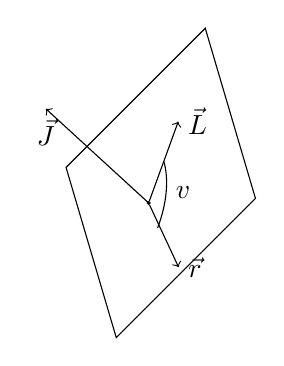
\begin{tikzpicture}[rotate around z=45, rotate around x=-45]
\draw (0,-0.3,0) -- (2.5,-0.3,0) -- (2.5,2.5,0) -- (0,2.5,0) -- cycle;
\draw[->] (1.,1.,0)node[draw,circle,inner sep=0] (o) {} -- (1.5,1.5,2)node[below] {$\vec{J}$};
\draw[->] (o) -- ++(295:0.9cm)node[right] {$\vec{r}$};
\draw[->] (o) -- ++(70:1.1cm)node[right] {$\vec{L}$}node [midway] (aux){};
\draw (aux) arc (0:-50:1) node[midway,right] {$v$};
\end{tikzpicture}

\label{fig:Lenztikz}

\end{figure}

\end{filecontents}

\begin{filecontents}{cylsang.tex}
    %\begin{tikzpicture}[tdplot_main_coords]
%%    \draw[-latex] (0,0,0) -- (1,0,0) node[pos=1.1]{$x$};
%%    \draw[-latex] (0,0,0) -- (0,1,0) node[pos=1.1]{$y$};
%%    \draw[-latex] (0,0,0) -- (0,0,1) node[pos=1.1]{$z$};
%  \begin{scope}[canvas is xy plane at z=0]
%   \path (0,0) coordinate[label=below:$O$] (O);
%   \draw[dashed] (\tdplotmainphi:\myr) arc(\tdplotmainphi:\tdplotmainphi+180:\myr);
%   \draw[dashed] (\angA:\myr) coordinate (A) -- (\angB:\myr) coordinate (B)
%    node[pos=-0.1] {$A$} node[pos=1.1] {$B$};
%   \draw[thick] (\tdplotmainphi:\myr) coordinate(BR) arc(\tdplotmainphi:\tdplotmainphi-180:\myr)
%   coordinate(BL);
%  \end{scope} 
\begin{axis}[
axis lines=center,
axis on top,
every inner z axis line/.append style={opacity=0},
xlabel={$x$}, ylabel={$y$}, zlabel={$t$},
domain=0:1,
y domain=0:2*pi,
xmin=-1.5, xmax=1.5,
ymin=-1.5, ymax=1.5, zmin=0.0,zmax=1.2,ztick={1},
every axis x label/.style={at={(rel axis cs:0,0.5,0)},anchor=south},
every axis y label/.style={at={(rel axis cs:0.5,0,0)},anchor=north},
every axis z label/.style={at={(rel axis cs:0.5,0.5,0.9)},anchor=west},
samples=30]
\addplot3 [surf, colormap/blackwhite, shader=flat] ({x*cos(deg(y))},{x*sin(deg(y))},{x});
\addplot3 [domain=0:360,samples y=1,name path=top,draw=none] ({1*cos(deg(x))},{1*sin(deg(x))},{1});
\path[name path=zline] (0,0,0) -- (0,0,1.2) coordinate(ztop);
\path[name intersections={of=top and zline,by={aux1}}];
\draw[-latex] (aux1) -- (ztop);
%standard tikz coordinate definition using x, y, z coords
\coordinate (O) at (0,0,0);

%tikz-3dplot coordinate definition using x, y, z coords
%\pgfmathsetmacro{\axone}{0.5}
%\pgfmathsetmacro{\ayone}{0.3}
%\pgfmathsetmacro{\azone}{0.4}
%\pgfmathsetmacro{\axtwo}{0.3}
%\pgfmathsetmacro{\aytwo}{0.5}
%\pgfmathsetmacro{\aztwo}{0}
%\coordinate (P1) at (\axone,\ayone,\azone);
%\coordinate (P2) at (\axtwo,\aytwo,\aztwo);
%\coordinate (P3) at (\axone+\axtwo,\ayone+\aytwo,\azone+\aztwo);
%\fill[red,opacity=0.2] (O) -- (P1) -- (P3) -- (P2) -- cycle;
%\draw[vector] (O) -- (P1);
%\draw[vector] (O) -- (P2);
\addplot3[
    samples y=0,
    smooth, thick, color=blue,
    domain=0:sqrt(2)
    ] ({0},{4-2*x^2},{x}) coordinate [pos=0.3] (trihedron origin) ;
\draw [-latex,color=violet,thick] (trihedron origin) -- +(axis direction cs:0,0,1)
    node [anchor=west] {$ds$};
\end{axis}
\end{filecontents}
%%contain tikz files as filecontents
\addtolength{\textheight}{-0pt}
\addtolength{\headheight}{0pt}
\addtolength{\footskip}{0pt}


% Section and subsections will appear in the presentation overview
% and table of contents.
%\frame{\tableofcontents[onlyparts]}

\begin{frame}[fragile]{Fisica stellare: argomenti del corso}%label={}
    %\framesubtitle{Main onlyparts TOC}
   %\begin{columns}[T]%list of frame a inizio sezione
    % \begin{column}{0.45\textwidth}
    \tableofcontents[onlyparts]
    %    \end{column}
      %  \begin{column}{0.55\textwidth}
      %      \listofcherryframes
      %  \end{column}
   % \end{columns}
\end{frame}

\begin{frame}{Fisica stellare: i frames pi\'u importanti}%label={}
     \listofcherryframes
\end{frame}

\begin{frame}{Meta}
    argomenti del corso: toc parts a sinistra e important frames a destra
    todo, must: before reglez; frame importanti
    listofframe all'inizio di ogni sezione per frames con sottotitolo
frameinlbftrue: listofcherryframes
\end{frame}

\begin{frame}{Perch\'e studio queste cose?? Sviluppi; futuro.}
Concretezza, concentrazione, indipendenza
\end{frame}

\part{Intro}%\linkdest{intro}
%! TEX root = main.tex
\section{Fonti}

\begin{wordonframe}{Lectures: 29/09/2022}
    \begin{block}{Atomic level population and photon gas}
        \begin{columns}[T]
            \begin{column}{0.5\textwidth}
                \begin{itemize}
                    \item Stimulated de-exc: $n_jB_{ji}I_{\nu}\phi_{em}$
                    \item Stimulated excitation: $n_iB_{ij}I_{\nu}\phi_{abs}$
                \end{itemize}<++>
            \end{column}
            \begin{column}{0.5\textwidth}
                <++>
            \end{column}
        \end{columns}
        <++>
    \end{block}<++>

\end{wordonframe}

\section{RegLez: Processi settembre 2022 (22/23)}\linkdest{rl22}

\begin{frame}[allowframebreaks]{List of todos}
\listoftodos
\end{frame} 

\begin{frame}[allowframebreaks]{List of Keywords}
\listofkeywords
\end{frame}    

\begin{frame}[allowframebreaks]{List of Musts}
\listofmusts
\end{frame}


\begin{frame}[allowframebreaks]{Reglez 22/23: Shore}
    \begin{itemize}
\item 04/09/2022 Formal solution to the \keyword{transfer equation}; moments of the intensity; curvature effects (outline); scattering and source function; light echos as a scattering problem 
\item 20/09/2022 Introduction to the course: objectives, main references and description of the exam. Observation vs experiment. Fundaments of spectral formation and interaction between photons and a medium.
\item 22/09/2022 Diffusion equation, intensity and flux. Formal transfer equation. Absorption and scattering coefficients. Source function. Non linearity of the transfer equation. Two level atom: Einsteins coefficients and radiative equilibrium condition. Generic form of the source function. 
\item 27/09/2022 Definition of Local thermodynamic equilibrium (LTE). Hypothesis of complete redistribution and source function. Relation between Einstein's coefficients at LTE and Planck distribution. Collisional balance and detailed balance. Non-LTE and radiation feedback on populations. Ionisation balance and Saha Equation for LTE. 
\item 29/09/2022 Hydrostatic equilibrium as the basis of atmospheric structure (interchanges between pressure, optical deepth, geometric depth, and viewing angle), the context of the inverse radiative transfer problem (spectroscopic recovery of the thermal structure of an atmosphere, the importance of a spectrum relative to filter photometry); equation of transfer (2), beginnings of formal solution. 
\item 04/10/2022 Moments of the transfer equation, radiative equilibrium; inverse problem 
\item 06/10/2022 Moments of the transfer equation and closure (Eddington approximation) in diffusive limit; definition of mean opacity and the specifics of the Rosseland mean opacity; electron scattering; bremsstrahlung; H- and the stratification of opacity in stellar interiors (and the importance of matching the source function peak to that of the opacity); radiative forcing and climate change as an example of diffusive transport. 
\item 11/10/2022 Mean opacity and frequency dependence leading to temperature dependence (Kramers' opacity as an example). Line spectra: atomic states, intrinsic broadening, profile function (convolutions), line opacity 
\item 13/10/2022 Zeeman effect on line foration, coherence, second solar spectrum (implicitly, the Hanle effect); Stark broadening, depression of the continuum and changes in equation of state and partition function; line driving for radiation pressure (and a mention of radiative driven diffusion); H II regions (1) 
\item 18/10/2022 Fluorescence, Rayleigh and Raman scattering, last pass on NLTE processes and line formation, radiative coupling. Beginning discussion of fluids, phase space and distrubution function and the evolution equation at microscopic level (fine/coarse graining). Continuity equation and introductory remarks. 
\item 20/10/2022 Forces acting on a fluid: body forces and interface forces. Stress tensor and definition of pressure as the isotropic part of the stress tensor. Fluids in equilibrium, hydrostatic equilibrium in spherical symmetry, vertically stratified atmosphere. Effect of rigid body rotation. Definition of vorticity. Streamlines, streaklines and vortex lines. 
\item 25/10/2022 Participation to the seminar: ``Superfluids from the cosmos to the lab: from vortices in neutron stars and quark matter to searches for the neutron electric dipole moment and low mass dark matter'' by prof. Baym. Follow up discussion and comments: circulation and conservation of circulation in ideal fluids. Vortex pinning. Determination of masses and radii of neutron stars and current constraints. 
\item 27/10/2022 More on vorticity and circulation. Conservation of circulation in ideal incompressible fluids. Evolution equation for the vorticity. Navier-Stokes equation, Reynolds number and qualitative discussion of turbulence. De Laval nozzle and super-sonic motion, qualitative correspondence with stellar wind solutions. Acoustic waves from pressure perturbations. Definition of the speed of sound. 
\item 03/11/2022 Sound (again, with breaking conditions); astero-helioseismology and standing waves with random excitation; esxtension to a pressure gradient driven wind (Parker solution) with gravity (solar wind) and critical radius (escape); radiative driving and winds from massive stars as extensions of the theory; P Cyg profiles and dynamical instability of line driven flows in the presence of sound waves. 
\item 08/11/2022 Instabilities: sound in a stratified atmosphere, buoyant instabilities; start on shear instabilities 
\item 10/11/2022  \todo{Shear instabilities} and applications; vorticity cascade and nonlinear development; turbulence - I 
\item 15/11/2022 \must{Kolmogorov theory}, cascade and turbulence - II 
\item 17/11/2022 Rotation in fluids
\item 22/11/2022 R ayleigh stability criterion for rotating fluids. Stability of Keplerian motion and epicyclic frequency. Diffusion of vorticity due to viscosity in Keplerian rings. Accretion discs: structure of a thin, Keplerian disc, pressure scale height and alpha-viscosity model. Shakura-Sunyaev thin disc. 
\item 24/11/2022 Shakura-Sunyaev thin disc solution. Temperature structure. Effect of radiation pressure in the inner regions of the disc. Eddington accretion rate. 
\item 29/11/2022 Similarity solutions and Buckingham PI theorem. Application to the Sedov-Taylor shock wave solution and its physical consequences (optical depth and adiabaticity). Rankine-Hugoniot junction conditions in planar shocks. Adiabatic vs isothermal shocks. 
\item 01/12/2022 Ionisation fronts. Reionisation. Active galactic nuclei and their classification. Question time.                                                                       \item 06/12/2022 More on self-similarity and self-similar solutions. The structure of a post-shock fluid. Introduction to gravitational waves: quadrupole formula and flash from merging binaries. Historic development of the theory and phenomenological description of the coalescence process. 
\item 13/12/2022 Sources of gravitational waves and their main characteristics: transient and continuous. Coalescence of compact binaries. Quadrupolar emission pattern and selection effects in gravitational wave astronomy. Overview of current catalogs of coalescing binaries. 
\end{itemize}
\end{frame}

\begin{wordonframe}{RegLez 22/23: Del Pozzo}
    \begin{itemize}
\item  04/09/2022 Formal solution to the transfer equation; moments of the intensity; curvature effects (outline); scattering and source function; light echos as a scattering problem 
\item 20/09/2022 Introduction to the course: objectives, main references and description of the exam. Observation vs experiment. Fundaments of spectral formation and interaction between photons and a medium. 
\item 22/09/2022 Diffusion equation, intensity and flux. Formal transfer equation. Absorption and scattering coefficients. Source function. Non linearity of the transfer equation. Two level atom: Einsteins coefficients and radiative equilibrium condition. Generic form of the source function. 
\item 27/09/2022 Definition of Local thermodynamic equilibrium (LTE). Hypothesis of complete redistribution and source function. Relation between Einstein's coefficients at LTE and Planck distribution. Collisional balance and detailed balance. Non-LTE and radiation feedback on populations. Ionisation balance and Saha Equation for LTE. 
\item 29/09/2022 Hydrostatic equilibrium as the basis of atmospheric structure (interchanges between pressure, optical deepth, geometric depth, and viewing angle), the context of the inverse radiative transfer problem (spectroscopic recovery of the thermal structure of an atmosphere, the importance of a spectrum relative to filter photometry); equation of transfer (2), beginnings of formal solution. 
\item 04/10/2022 Moments of the transfer equation, radiative equilibrium; inverse problem 
\item 06/10/2022 Moments of the transfer equation and closure (Eddington approximation) in diffusive limit; definition of mean opacity and the specifics of the Rosseland mean opacity; electron scattering; bremsstrahlung; H- and the stratification of opacity in stellar interiors (and the importance of matching the source function peak to that of the opacity); radiative forcing and climate change as an example of diffusive transport. 
\item 11/10/2022 Mean opacity and frequency dependence leading to temperature dependence (Kramers' opacity as an example). Line spectra: atomic states, intrinsic broadening, profile function (convolutions), line opacity 
\item 13/10/2022 Zeeman effect on line foration, coherence, second solar spectrum (implicitly, the Hanle effect); Stark broadening, depression of the continuum and changes in equation of state and partition function; line driving for radiation pressure (and a mention of radiative driven diffusion); H II regions (1) 
\item 18/10/2022 Fluorescence, Rayleigh and Raman scattering, last pass on NLTE processes and line formation, radiative coupling. Beginning discussion of fluids, phase space and distrubution function and the evolution equation at microscopic level (fine/coarse graining). Continuity equation and introductory remarks. 
\item 20/10/2022 Forces acting on a fluid: body forces and interface forces. Stress tensor and definition of pressure as the isotropic part of the stress tensor. Fluids in equilibrium, hydrostatic equilibrium in spherical symmetry, vertically stratified atmosphere. Effect of rigid body rotation. Definition of vorticity. Streamlines, streaklines and vortex lines. 
\item 25/10/2022 Participation to the seminar: ``Superfluids from the cosmos to the lab: from vortices in neutron stars and quark matter to searches for the neutron electric dipole moment and low mass dark matter'' by prof. Baym. Follow up discussion and comments: circulation and conservation of circulation in ideal fluids. Vortex pinning. Determination of masses and radii of neutron stars and current constraints. 
\item 27/10/2022 More on vorticity and circulation. Conservation of circulation in ideal incompressible fluids. Evolution equation for the vorticity. Navier-Stokes equation, Reynolds number and qualitative discussion of turbulence. De Laval nozzle and super-sonic motion, qualitative correspondence with stellar wind solutions. Acoustic waves from pressure perturbations. Definition of the speed of sound. 
\item 03/11/2022 Sound (again, with breaking conditions); astero-helioseismology and standing waves with random excitation; esxtension to a pressure gradient driven wind (Parker solution) with gravity (solar wind) and critical radius (escape); radiative driving and winds from massive stars as extensions of the theory; P Cyg profiles and dynamical instability of line driven flows in the presence of sound waves. 
\item 08/11/2022 Instabilities: sound in a stratified atmosphere, buoyant instabilities; start on shear instabilities 
\item 10/11/2022 Shear instabilities and applications; vorticity cascade and nonlinear development; turbulence - I 
\item 15/11/2022 Kolmogorov theory, cascade and turbulence - II 
\item 17/11/2022 Rotation in fluids 
\item 22/11/2022 Rayleigh stability criterion for rotating fluids. Stability of Keplerian motion and epicyclic frequency. Diffusion of vorticity due to viscosity in Keplerian rings. Accretion discs: structure of a thin, Keplerian disc, pressure scale height and alpha-viscosity model. Shakura-Sunyaev thin disc. 
\item 24/11/2022 Shakura-Sunyaev thin disc solution. Temperature structure. Effect of radiation pressure in the inner regions of the disc. Eddington accretion rate. 
\item 29/11/2022 Similarity solutions and Buckingham PI theorem. Application to the Sedov-Taylor shock wave solution and its physical consequences (optical depth and adiabaticity). Rankine-Hugoniot junction conditions in planar shocks. Adiabatic vs isothermal shocks. 
\item 01/12/2022 Ionisation fronts. Reionisation. Active galactic nuclei and their classification. Question time. 
\item 06/12/2022 More on self-similarity and self-similar solutions. The structure of a post-shock fluid. Introduction to gravitational waves: quadrupole formula and flash from merging binaries. Historic development of the theory and phenomenological description of the coalescence process. 
\item 13/12/2022 Sources of gravitational waves and their main characteristics: transient and continuous. Coalescence of compact binaries. Quadrupolar emission pattern and selection effects in gravitational wave astronomy. Overview of current catalogs of coalescing binaries. 
\end{itemize}

\end{wordonframe}


%! TEX root = main.tex
\section{Succo}\linkdest{succo}

\section{LTE}

\section{atmosphere}

\section{hydrostatic equilibrium}

\section{parker solution: wind and accretion}

\section{self-similarity}

\section{turbulence}

\section{Shock}

\part{Modello Plasma stellare}%\linkdest{stellarplasma}
\begin{frame}{this part toc}
    \begin{itemize}
        \item Recap recap stat phys gas of photons
        \item Radiative transfer equation and solution in far interior
        \item Recap atomic line light scattering
        \item Nuclear Fusion
    \end{itemize}
\end{frame}
\input{stellarplasmamodel}

\part{Modelli stellari: struttura ed evoluzione}%\linkdest{evolutivemodels}
\begin{frame}{this part toc}
%\begin{columns}[T]
%\begin{column}{0.5\textwidth}
\begin{itemize}
\item Eqs struttura stellare
\item Meccanismi di trasporto e stabilit\'a
\item Fenomenologia del plasma stellare
\item Luminosity production. Nuclear reactions
\item Metodi soluzione modello stellare
\end{itemize}
%\end{column}
%\begin{column}{0.5\textwidth}
%\tableofcontents
%\end{column}
%\end{columns}
\end{frame}
\input{starmodels}
 
  \part{Formazione ed evoluzione stellare} 
\begin{frame}{TOC formation evolution}
\tableofcontents
\end{frame}
\input{starformation}
\input{stellarevolution}
 
 \part{Stellar population in the milky way}%\linkdest{constraints}
\begin{frame}{this part toc}
\begin{columns}[T]
\begin{column}{0.5\textwidth}
\begin{itemize}
	\item Solar neighborhood
\end{itemize}
\end{column}
\begin{column}{0.5\textwidth}
\tableofcontents
\end{column}
\end{columns}
\end{frame}
\input{GalaxyStarImfPop}
  
\end{document}
